\subsection{Data Diversity}

Faults within the data are the second largest cause of errors \cite{nasa:stats}, with that in mind, it is sometimes not enough to execute different version of a software on the same data in order to get an acceptable output. Instead, data diversity might be required to ensure correct execution. Data diversity is an orthogonal method to the previously mentioned design diversity methods. It can be used on its own, or in combination with other fault tolerance methods.

\subsubsection{Failure Regions}

In many situations only very specific conditions will result in an error, we call these specific condition edge-cases. Even with thorough testing, there is no guarantee that all edge-cases will be caught during development, since the failure domain can be extremely small. We can take advantage of this, however, by using "reexpressed" input on a subsequent execution of a procedure, since even small adjustments of the input are likely to move it away from the failure domain. 

\subsubsection{Data Reexpression}

Data reexpression is generation of logically equivalent data sets. Any mapping of a program's data that preserves the information content of the data is a valid reexpression algorithm. A simple approximate data reexpression algorithm for a floating-point quantity might alter its value by a small percentage. The allowable percentage by which the data value could be altered would be determined by the application. In applications that process sensor data, for example, the accuracy of the data is often poor and deliberate small changes are unlikely to affect performance. \cite{nasa:datadiversity}

% \begin{figure}[hbt]
%     \centering
%     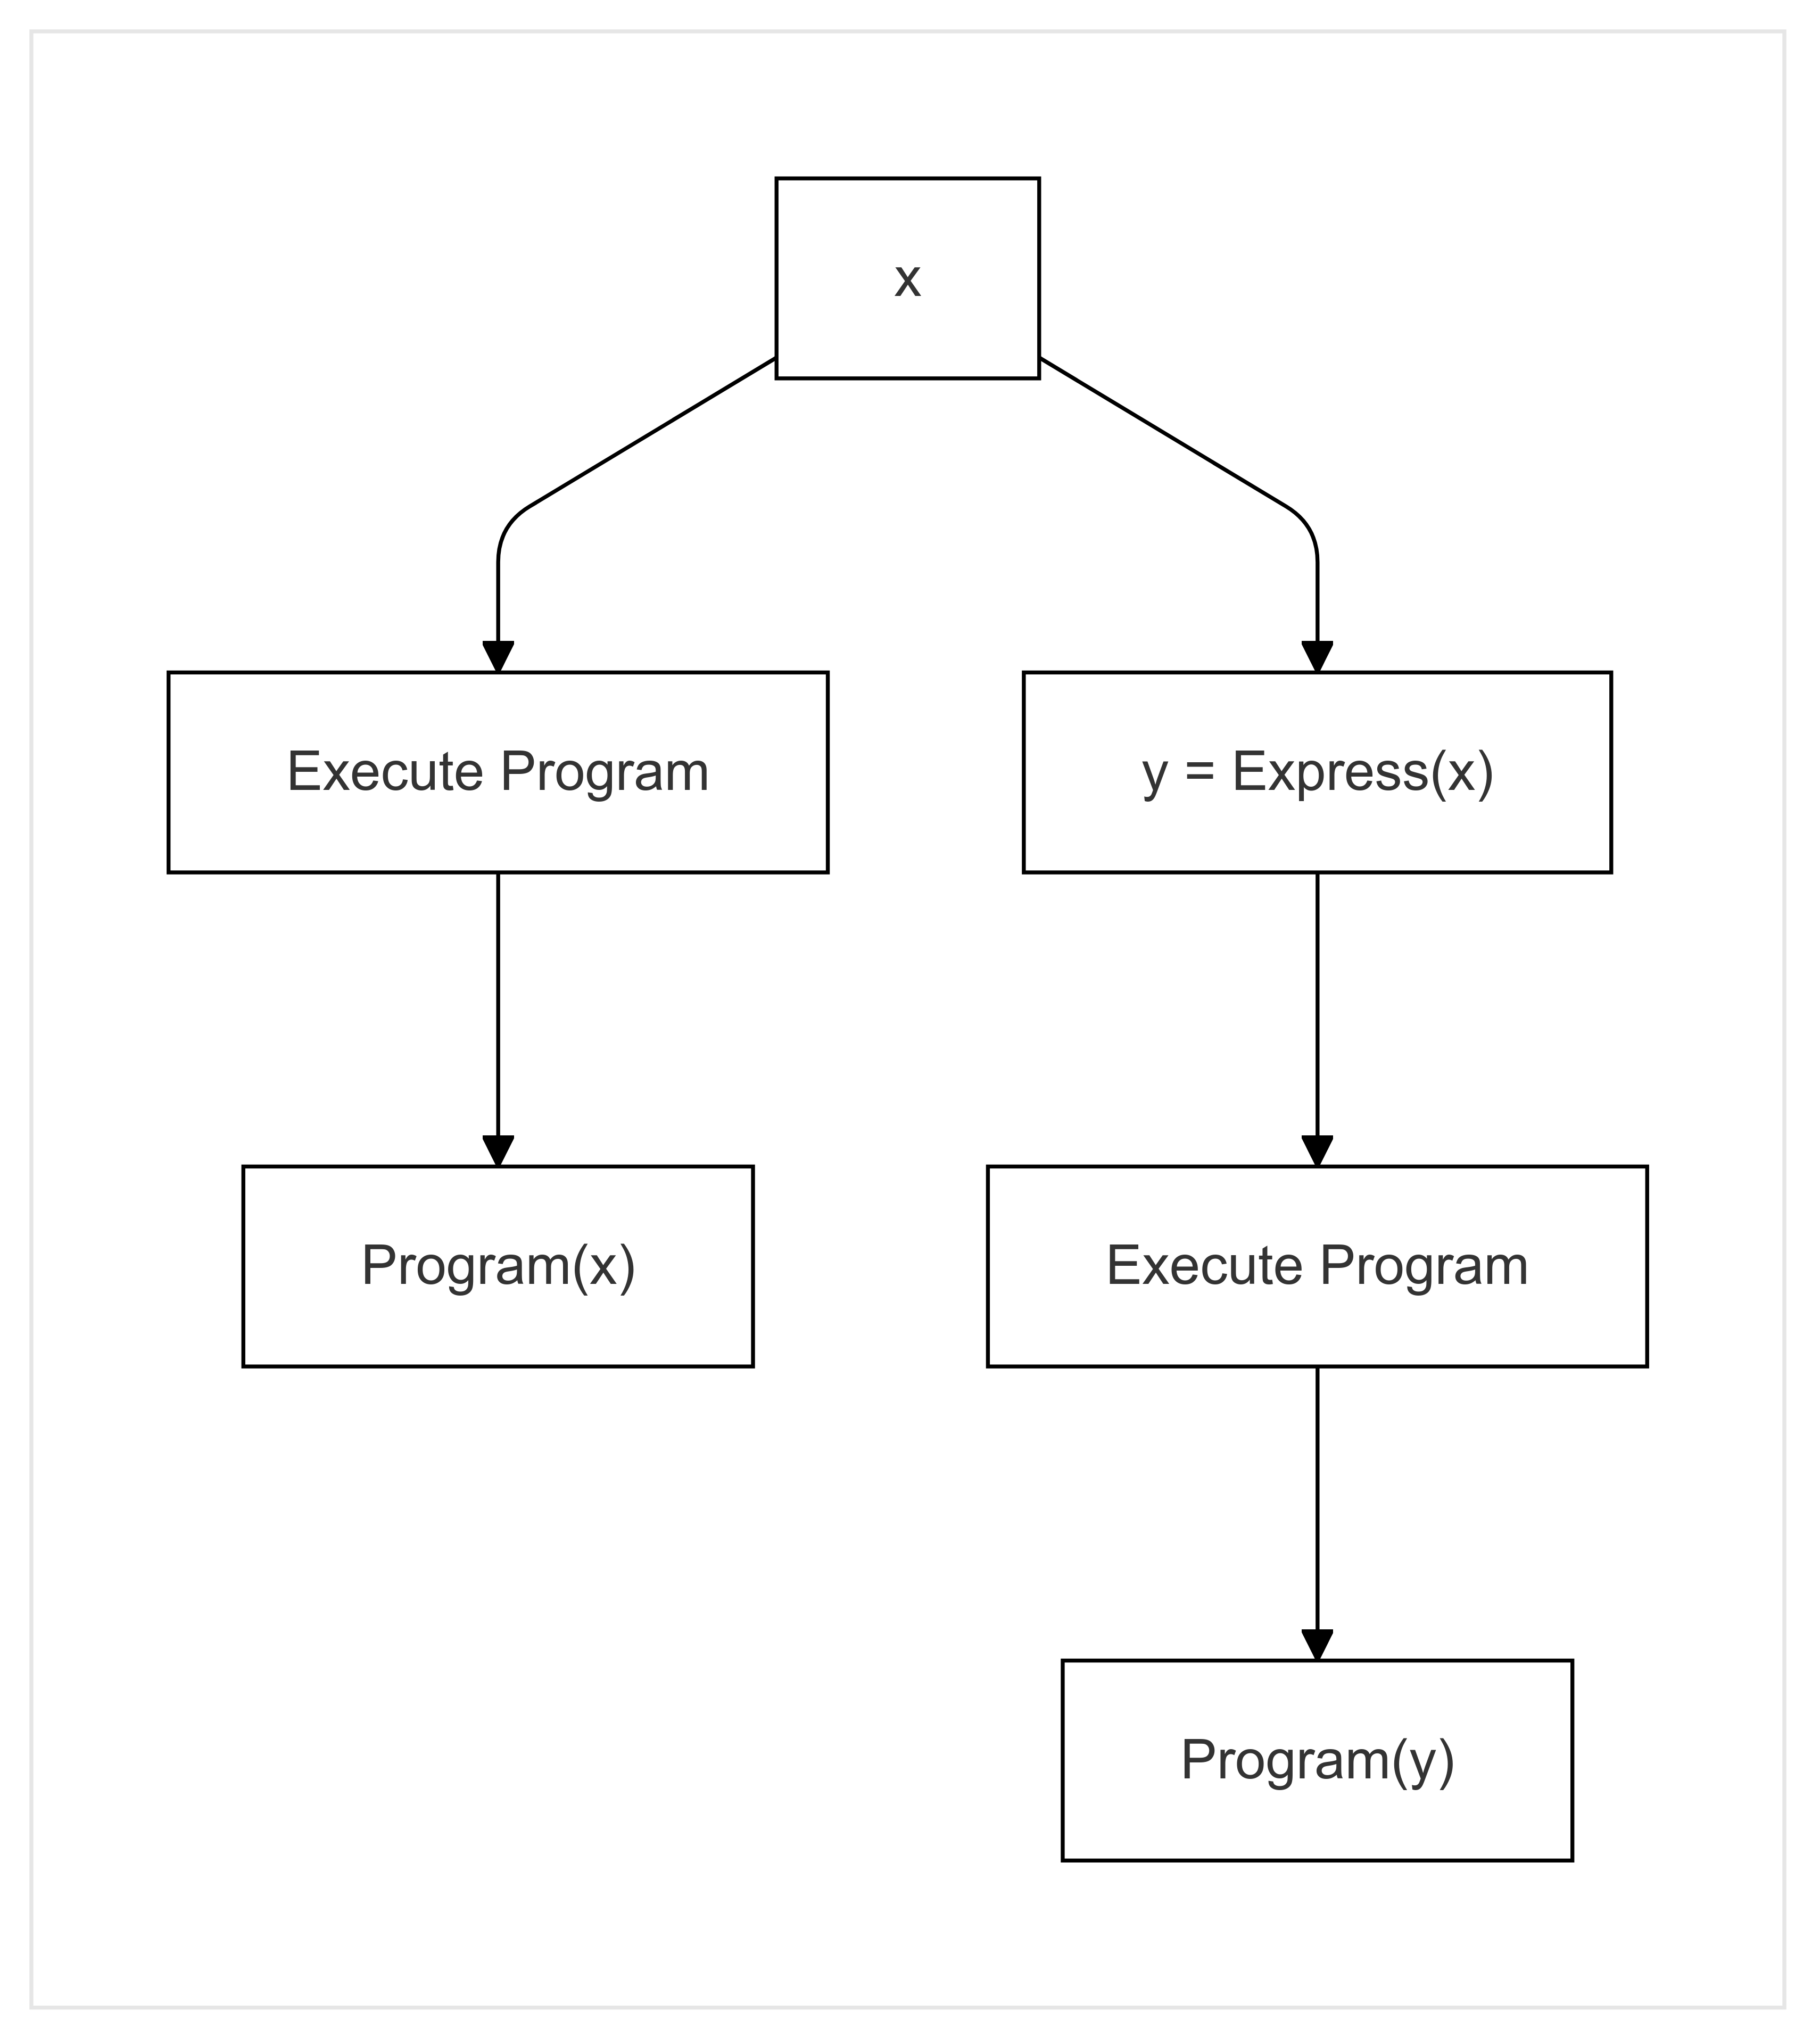
\includegraphics[width=0.7\textwidth]{diagrams/data_div/reexpress.png}
%     \caption{Data Reexpression}
%     \label{fig:data_rex}
% \end{figure}